\documentclass[12pt,a4paper]{report}
\usepackage{amsmath}
\usepackage{amsfonts}
\usepackage{amssymb}
\usepackage{graphicx}
\usepackage{multicol}
\usepackage[utf8]{inputenc}
\usepackage{array}
\usepackage{lipsum}
\graphicspath{{images/}}
\usepackage{parskip}
\usepackage{indentfirst}
\usepackage{courier}
\usepackage{titlesec}
\usepackage{wrapfig}
\usepackage{caption}
\usepackage{geometry}
\usepackage{float}
\geometry{headheight = 12pt}
\parindent 15pt
\parskip 2ex

\renewcommand{\listfigurename}{Figures}
\renewcommand{\listtablename}{Tables}

\titleformat{\chapter}[display]   
{\normalfont\huge\bfseries}{\chaptertitlename\ \thechapter}{20pt}{\Huge}   
\titlespacing*{\chapter}{0pt}{-50pt}{20pt}

\author{Jacob Spigle, Zachary Painter, David Akridge, Hunter Figueroa}
\title{Critical Encounters}
\begin{document}
	
\maketitle

\tableofcontents
	
\newpage
\chapter*{Introduction}
\stepcounter{chapter}
\addcontentsline{toc}{chapter}{Introduction}

Role-playing games are games where players act as their characters. Usually in person, around a table, and controlled by the players speaking their actions in turn. This might not always be done by speaking in-character, but rather by following this basic structure:

\begin{enumerate}
	\item The GM describes the environment.
	\item The players describe what they want to do.
	\item The GM narrates the results of the characters? actions.
\end{enumerate}

There are countless possible character, monster, and scenario possibilities when constructing a tabletop role-playing campaign, however, it is hard and sometimes impossible to sift through them all and find the perfect encounter. Not only that,  but once you commit to a game or role-playing decision you are forced to see it through to completion in order to retain the game?s continuity. Players get one chance to design their character at the very start of a session, and once they do, that character?s path cannot be meaningfully changed. Spending so much time working on a character, and then coming to the first session to find out that they are severely unprepared for the tasks they are presented can be harrowing. On the other side, the GM spends so much time outside of the game to prepare a story and encounters that challenge the Players, so when that GM accidentally wipes out the entire team of Player Characters (PCs) in one unbalanced encounter, or if the PCs simply walk through a fight that was meant to challenge them for the remainder of the session, the GM feels they have failed the PCs in presenting a good game.
\newpage
\chapter*{Proposed Solution}
\stepcounter{chapter}
\addcontentsline{toc}{chapter}{Proposed Solution}

This project presents a service that can be used by both GMs and players to test out their characters, encounters, team builds, or boss fights in a simulated environment. This will allow users to figure out just how well their creation holds up to the requirements that they have set for themselves. This project seeks to develop a service that follows the rules of the d20 Game System, and by allowing the player or GM to import their character's/monsters' statistics and equipment, they then can play against an automated opponent or opponents using that creation. To further enhance a user's ability to test and refine encounters and PCs, users will be able to upload and share their encounters to their public space where others can try their own creations' skills in that creator's setting.

\newpage
\chapter*{Broader Impact}
\stepcounter{chapter}
\addcontentsline{toc}{chapter}{Broader Impact}

Tabletop games bring people together in a world where physical interaction is often lost in lieu of digital communication. This project aims to supplement these interactions by making them more accessible to newer players, as well as help experienced players spend less time on pre-game preparation. This project has the potential to broaden the audience of an already quickly expanding pastime to younger players and DM's. Concepts in the realm of tabletop games are very easily understood by a younger audience, as their imagination and creativity can run free in such games. However, the threshold of understanding for the many rules and balances may prove a bit overzealous for this audience. Having a service that allows improves accessibility to newer players will also bleed into improving accessibility for younger players as well. Additionally, users who do not have a group to play with may find and form groups with other users with whom they have played and shared content with.
	
\newpage
\chapter*{Personal Interests}
\stepcounter{chapter}
\addcontentsline{toc}{chapter}{Personal Interests}
	\section{Jacob Spigle}
	\begin{wrapfigure}{r}{0\textwidth}
		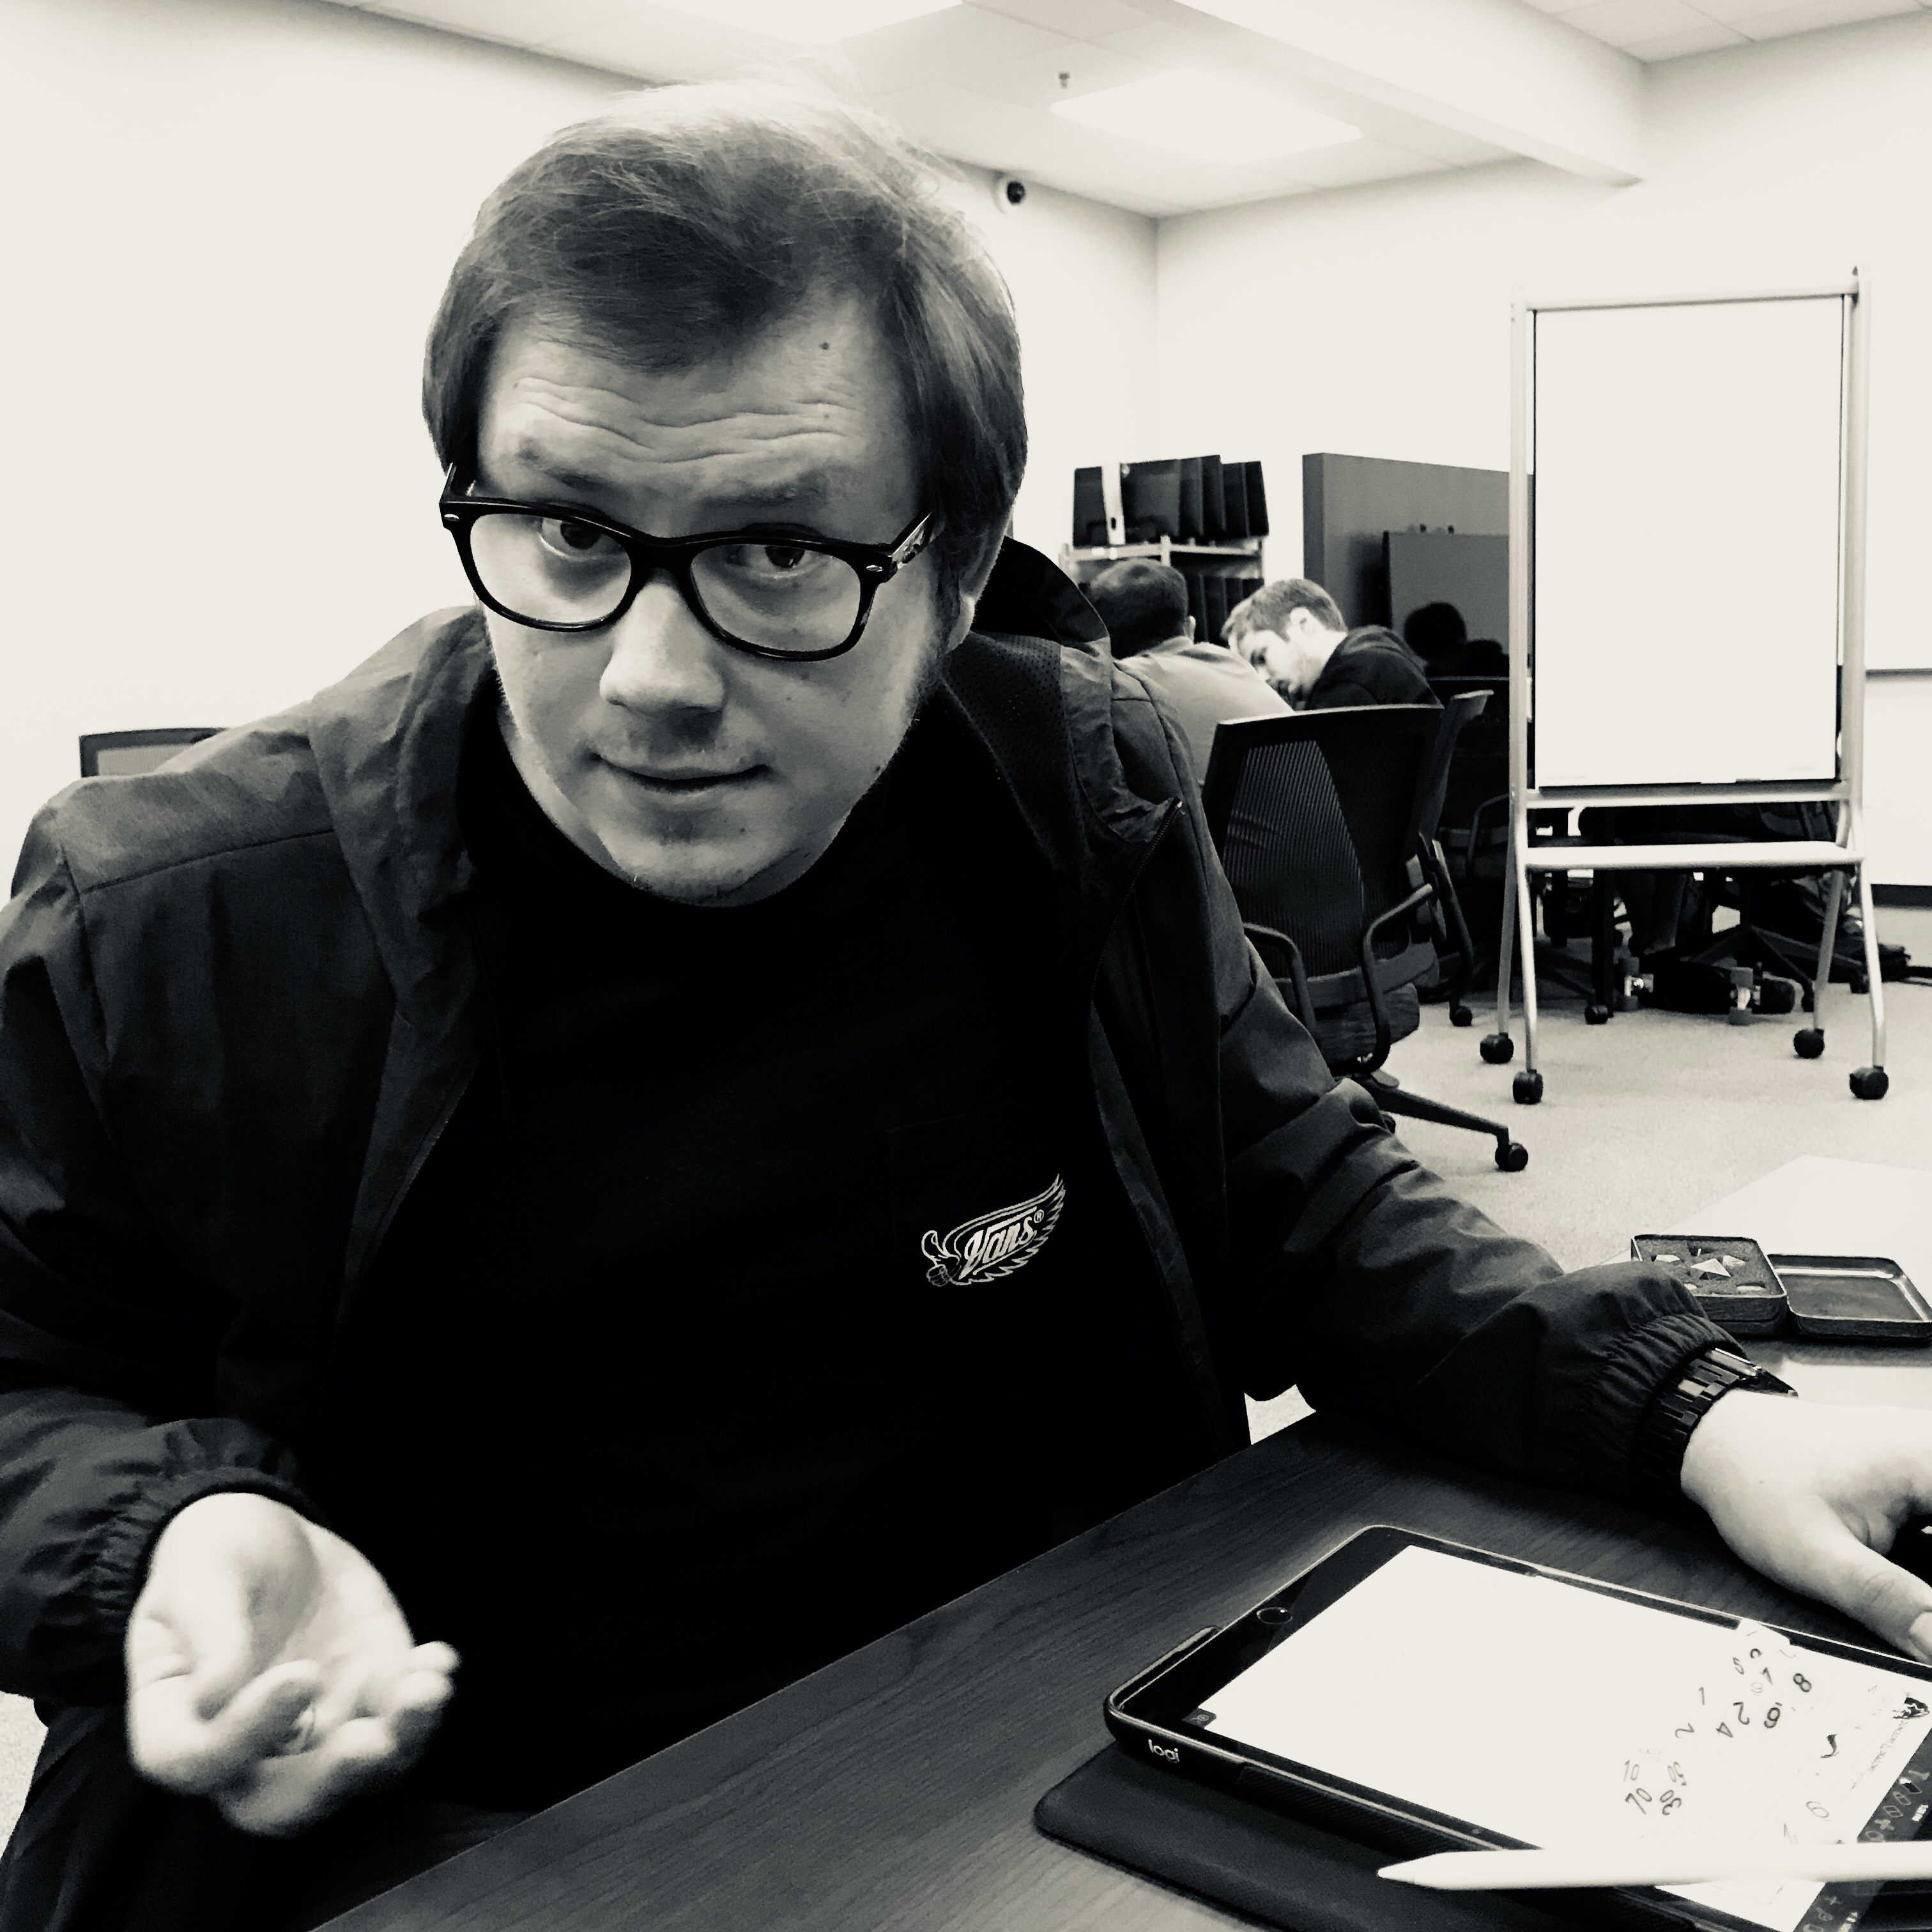
\includegraphics[scale=0.05]{Jacob_Spigle}
	\end{wrapfigure}
	I discovered role-playing games like Dungeons \& Dragons early this year. After playing video games since childhood, D\&D was a breath of fresh air; a way to mix the excitement of creating a character, leveling up, deciding your actions, along with an openness that allows nearly infinite stories, infinite worlds, and the tools to create those stories and worlds yourself. Those infinite possibilities can spur creations that might not work as well in-game as you thought. I have written campaigns and characters that on paper seemed great, but when brought to the table were found lacking. When I searched through the many different forums and groups I had joined after I started playing D\&D, and scouring the internet for a way to playtest my creations, I was surprised to found that no such tool existed. This service is something I can actually use and wish that I had during the creation of campaigns I have written, and that is why I believe others will find use in it as well.
	
	\newpage
	\section{Zachary Painter}
	\begin{wrapfigure}{l}{0\textwidth}
		
\includegraphics[scale=0.05]{Zachary_Painter}
	\end{wrapfigure}
	Some of my primary interests in Computer Science are data structures and algorithms. In my area of research, concurrent programming, these two topics are frequently discussed. Often times in this field, I have had the opportunity to explore many complicated and fascinating algorithms. When tackling these kinds of problems, you often find yourself spending considerably more time thinking and reasoning than implementing/coding. After understanding a problem, you move on to another without getting the chance to apply what you learned in a practical/usable way. This constant cycle of struggle/learn/get-new-problem is something that many students experience throughout college as they rarely have time to stop and demonstrate their rapidly growing skillset in a meaningful way. \par
	My motivation for being part of this project is that I want a chance to slow down and use the skills and algorithms I have picked up in my years at UCF in a useful and creative application instead of an abstract, un-impactful thought exercise. Instead of expecting this project to challenge me with highly complicated algorithms and difficult proofs, I expect this project to challenge me in project management skills, team coding, and the application of numerous techniques that I have learned but never had to implement in a meaningful way. There is an important difference between \textit{knowing} and \textit{doing}; and so I am taking this chance to remind myself what all my learning has amounted to. 
	
	\newpage
	\section{David Akridge}
	\begin{wrapfigure}{r}{0\textwidth}
		
\includegraphics[scale=0.05]{David_Akridge}
	\end{wrapfigure}
	This project caught my interest due to the combination of the creative nature of Dungeons \& Dragons mixed with the real world applications that can be gained by accomplishing the project’s end goal. In my time at UCF, we have learned tons of information primarily focusing on theories and concepts of computer science. While plenty of classes have had us working hands on, there is still much to learn before being able to stand out in the real world. This project is going to have us utilize the various algorithm implementations we’ve learned as well as diving into web development. As we haven’t covered web development in too far detail in the UCF curriculum, this project easily provides an opportunity for me to grasp the understanding of HTML, Javascript, Angular.js, etc. These are all languages and formats that I have had the desire the learn but lacked the drive to do on my own. \par
	Along with being able to learn practical CS skills, Critical Encounters will allow us to find creative workarounds be it code, web-page design, or even artwork. This is a really important aspect of the project to me, because many of the projects we’ve had to do prior have been numerically heavy and honestly not all that interesting. An engaging idea could help propel our ability to learn these new concepts, especially if we are interested in them on our own. Now that there is a great project motivating me and a great team to work alongside with, there is no doubt we will learn all the in’s and out’s of the subject. 
	
	\newpage
	\section{Hunter Figueroa}
	\begin{wrapfigure}{l}{0\textwidth}
		
\includegraphics[scale=0.05]{Hunter_Figueroa}
	\end{wrapfigure}
	I have been playing tabletop role-playing games for over 6 years now. They served as a creative outlet where I could experiment with new creative ideas. I prefer acting as a DM, I’ve only played a single session as a player, I loved the idea of being all powerful creator of a world that I could share with my friends. The tabletop community, namely the Dungeon \& Dragons community is like no other that I have seen before. It is composed of highly talented, highly cooperative  and interactive people who do their very best to better and expand the role playing community. For close to two years now I have put a considerable about of my free time into constructing a digital service to help this same cause. So when I heard Jacob pitch this idea, I knew it was the one for me. We’ve got something really special here, and with the team that we have I feel we can create something game changing.
	
\newpage
\chapter*{User Interface}
\stepcounter{chapter}
\addcontentsline{toc}{chapter}{User Interface}
	\section{Overall Design and Navigation Bar}
	The approach we took to user interface (UI) design was focused on a simplistic and familiar look and feel to allow for easy accessibility to new users while the website itself still retaining focus on the encounter tester. The template that website utilizes is reminiscent of the design that many social media sites take, for instance, sites like Twitter, Facebook, and YouTube.\par
	The site also uses the the single-page application structure that allows for easy traversal. The persistent navigation bar (Figure \ref{fig: NavBar}) has Critical Encounters' name and logo in the top left of each page which redirects users back to the homepage, a searchbar in the top of each page which redirects users to the Encounter Browser page, and the user's username in the top right of each page that links to the user's Arena.
	\bigskip
	\bigskip
	\begin{figure}[H]
		\centering
		\centerline{
\includegraphics[scale=.30]{navbar}}
		\caption{NavBar}
		\label{fig: NavBar}
	\end{figure}
	\section{Registration Page}
	\begin{figure}
		\centering
		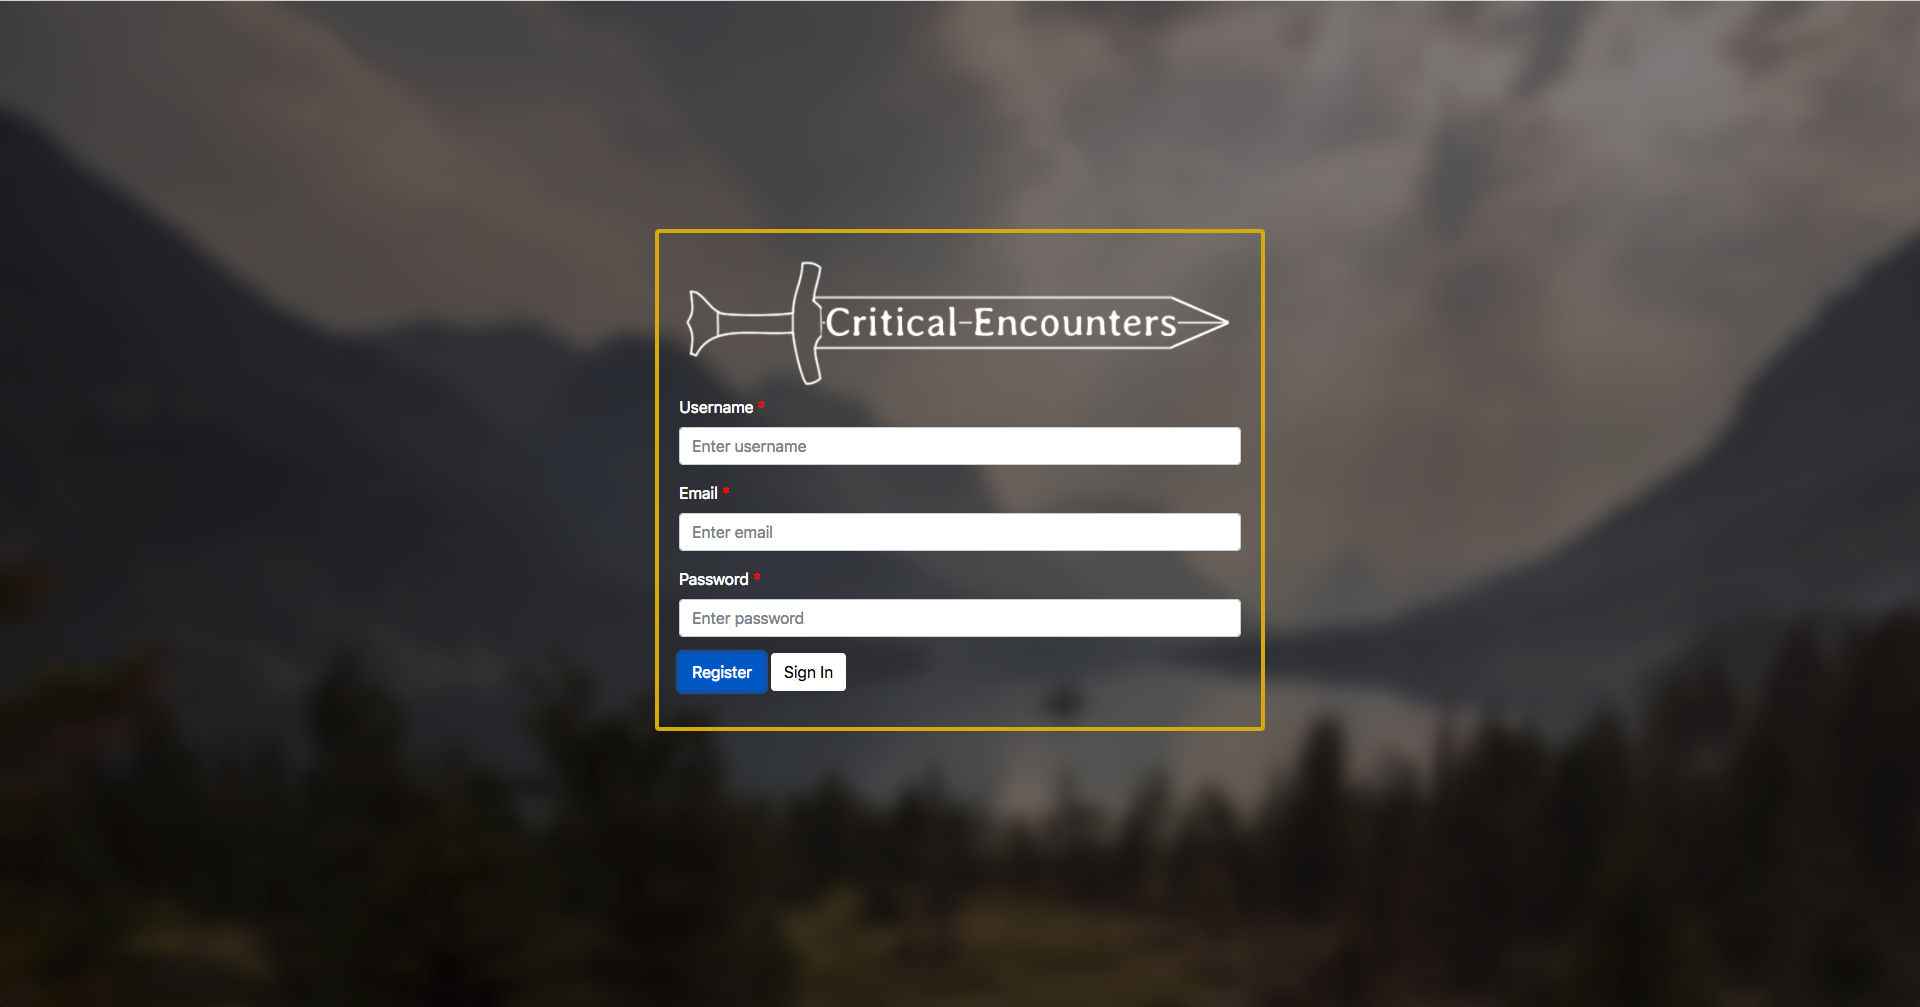
\includegraphics[scale=.20]{register}
		\caption{Registration Page}
		\label{fig: Registration Page}
	\end{figure}
	The registration page (Figure \ref{fig: Registration Page})  for Critical Encounters requires the user's desired username, their email addresss, and their password.
	\section{Login Page}
	\begin{figure}
		\centering
		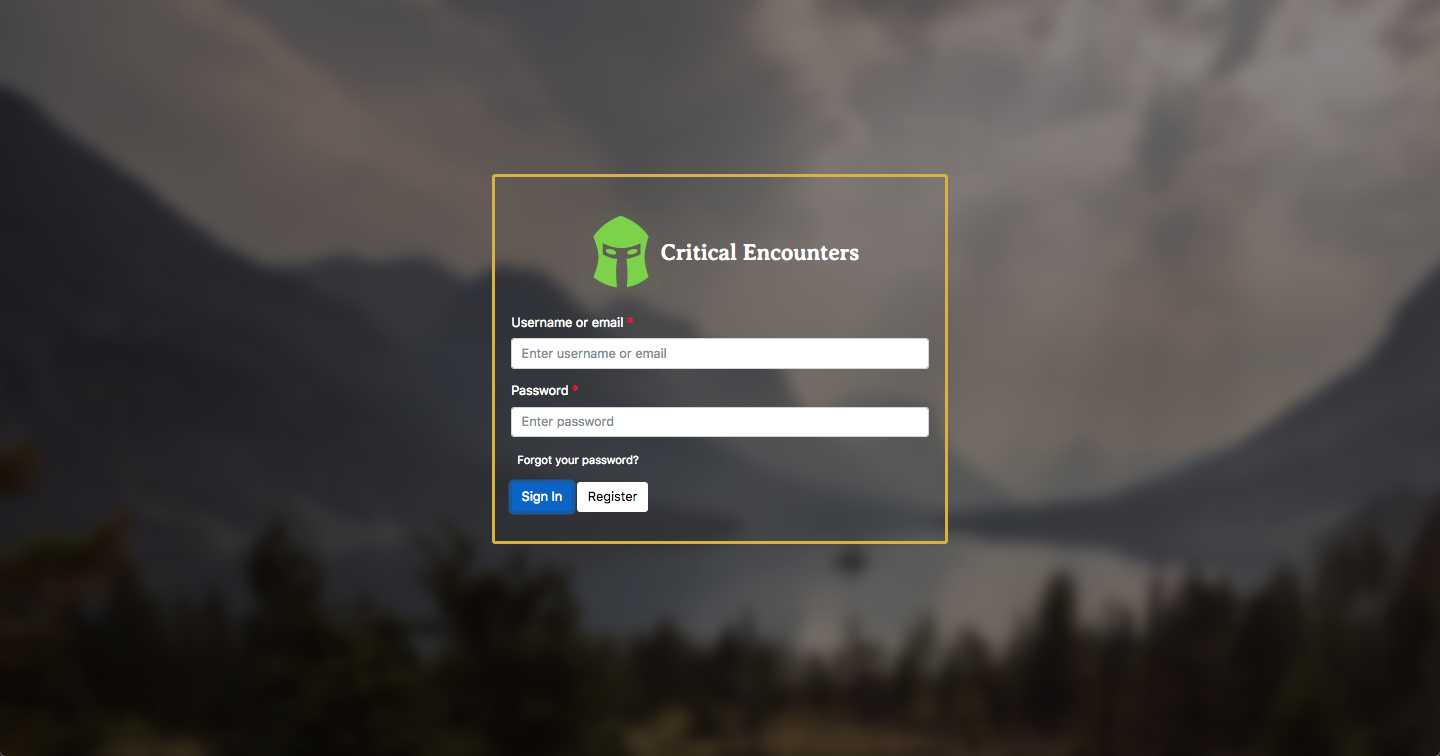
\includegraphics[scale=.20]{login}
		\caption{Login Page}
		\label{fig: Login Page}
	\end{figure}
	The login page (Figure \ref{fig: Login Page}) for Critical Encounters requires the user to enter either their username or email address along with the password tied to that account.
	\newpage
	\section{Dashboard}
	\begin{figure}[H]
		\centering
		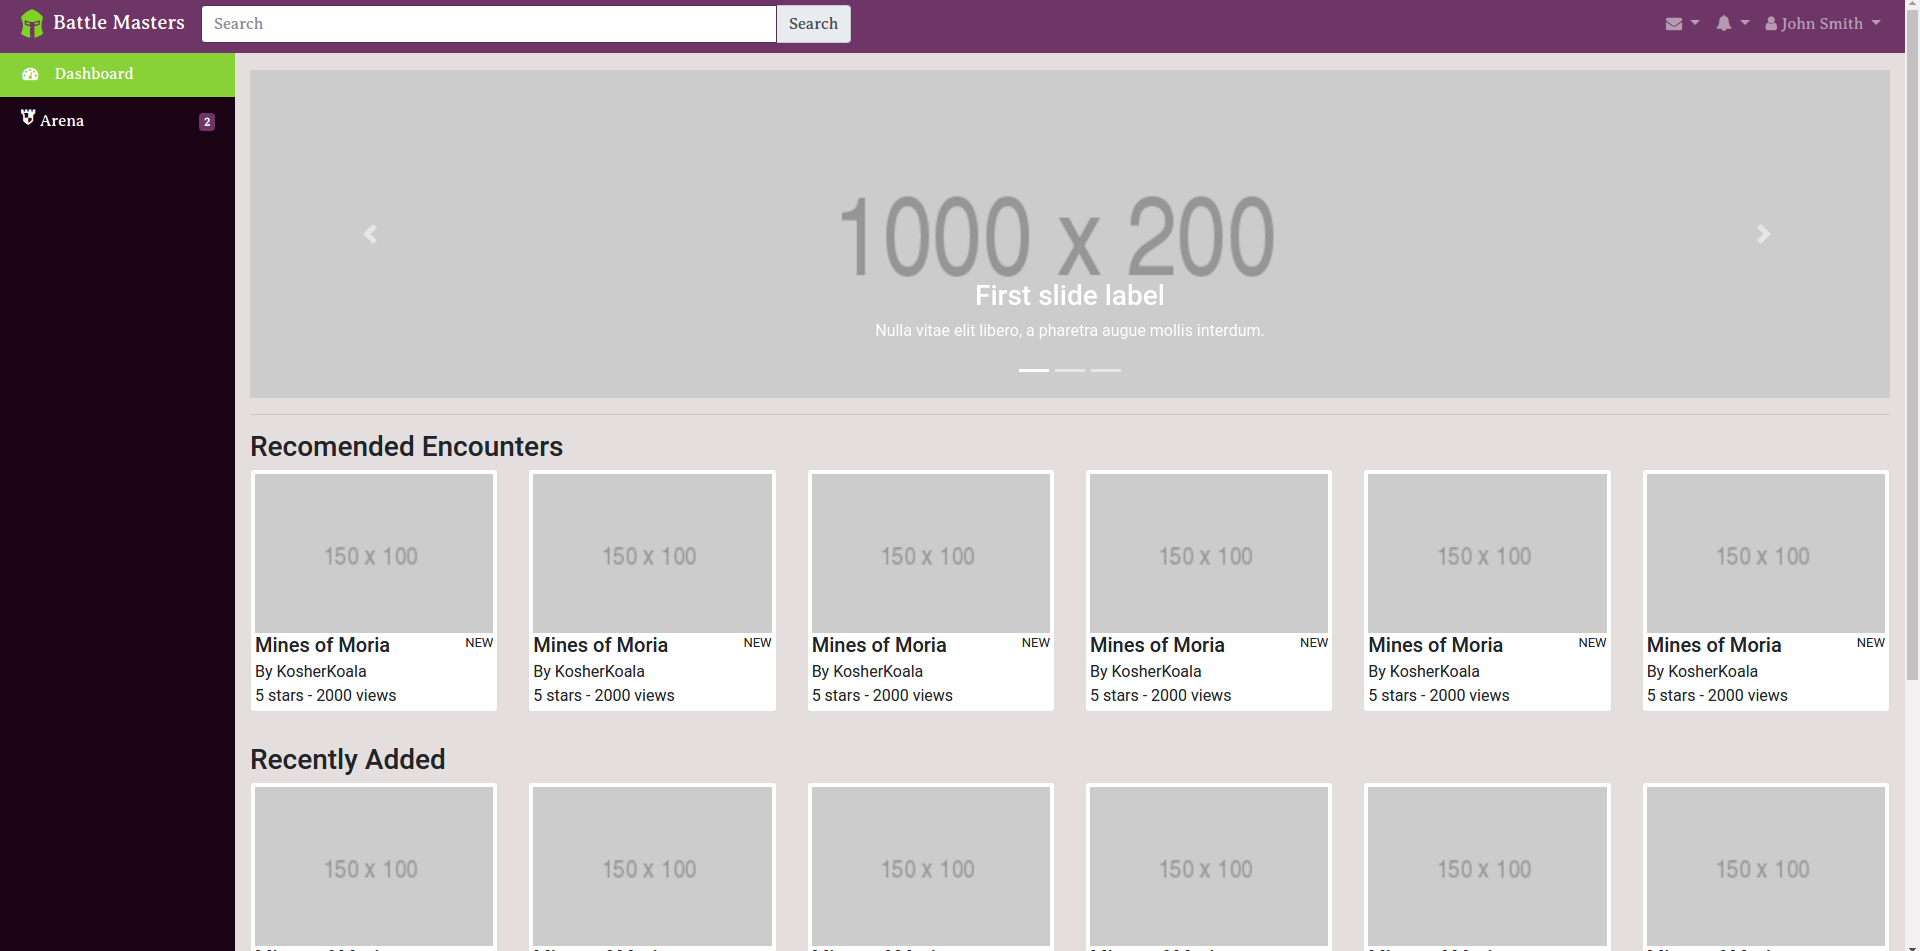
\includegraphics[scale=.20]{home}
		\caption{Dashboard}
		\label{fig: Dashboard}
	\end{figure}
	The Critical Encounters' Dashboard (Figure \ref{fig: Dashboard})features notable encounters, updates, and community events in the highlight wheel at the forefront of the page. Below the highlight wheel is a list of recommended encounters that either we the developers suggest to the community, or recommended list that is influenced by the user's recent search history.
	\section{Encounter Browser}
	\begin{figure}[H]
		\centering
		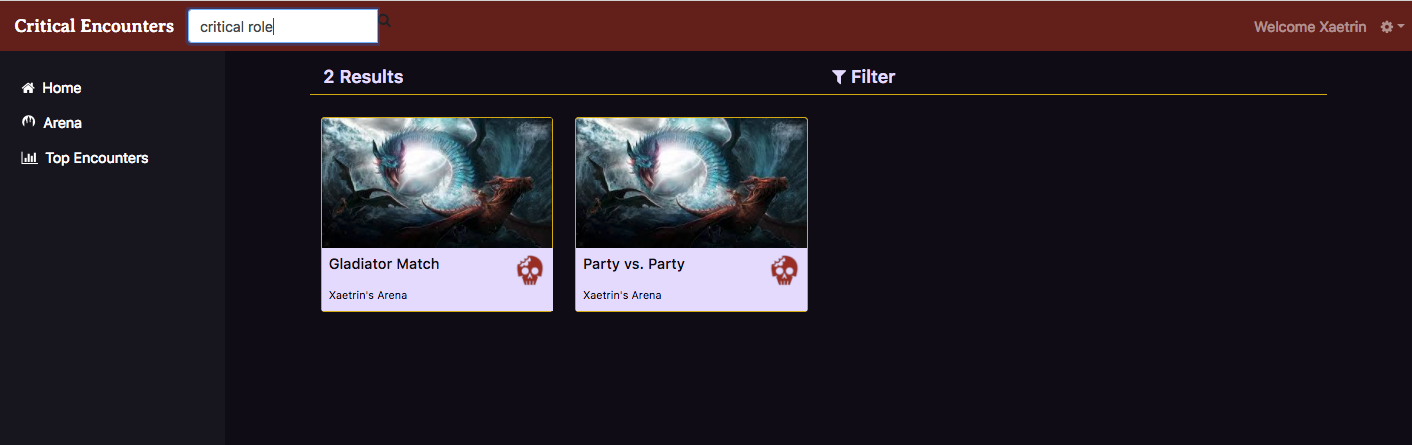
\includegraphics[scale=.20]{search}
		\caption{Encounter Browser}
		\label{fig: Encounter Browser}
	\end{figure}
	The Critical Encounters' Encounter Browser (Figure \ref{fig: Encounter Browser})acts as a search results page for queries entered in the searchbar in the navbar. From this page a list of filtered encounters is presented to the user. The user may also filter those results further by selecting settings from the dropdown menu revealed by the 'Filter' button. Through this process we can be sure to provide users with encounters that help with creation or simply encounters that help spark their own imagination. (Figure \ref{fig: Encounter Browser with Filter Options}).
	\begin{figure}[H]
		\centering
		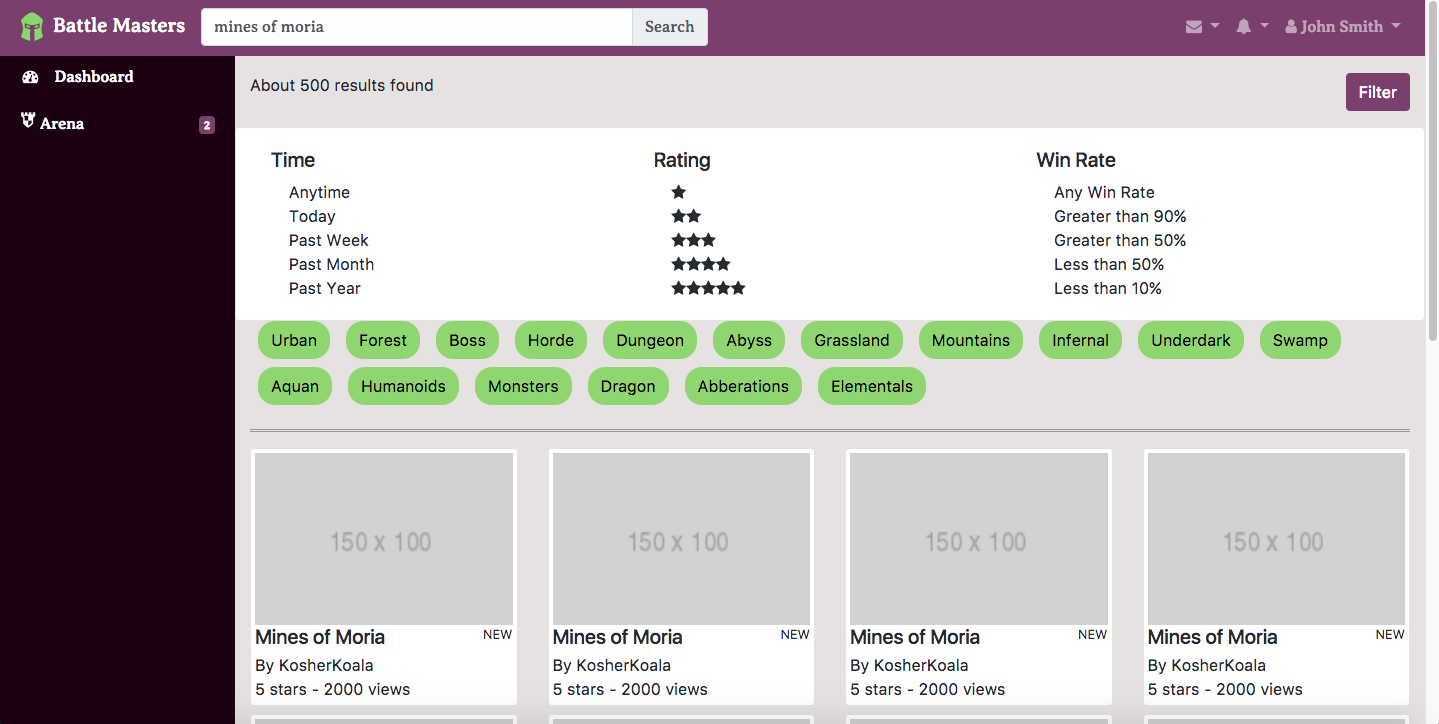
\includegraphics[scale=.27]{search_filtered}
		\caption{Encounter Browser with Filter Options}
		\label{fig: Encounter Browser with Filter Options}	
	\end{figure}
	\newpage
	\section{Arena}
	\begin{figure}[H]
		\centering
		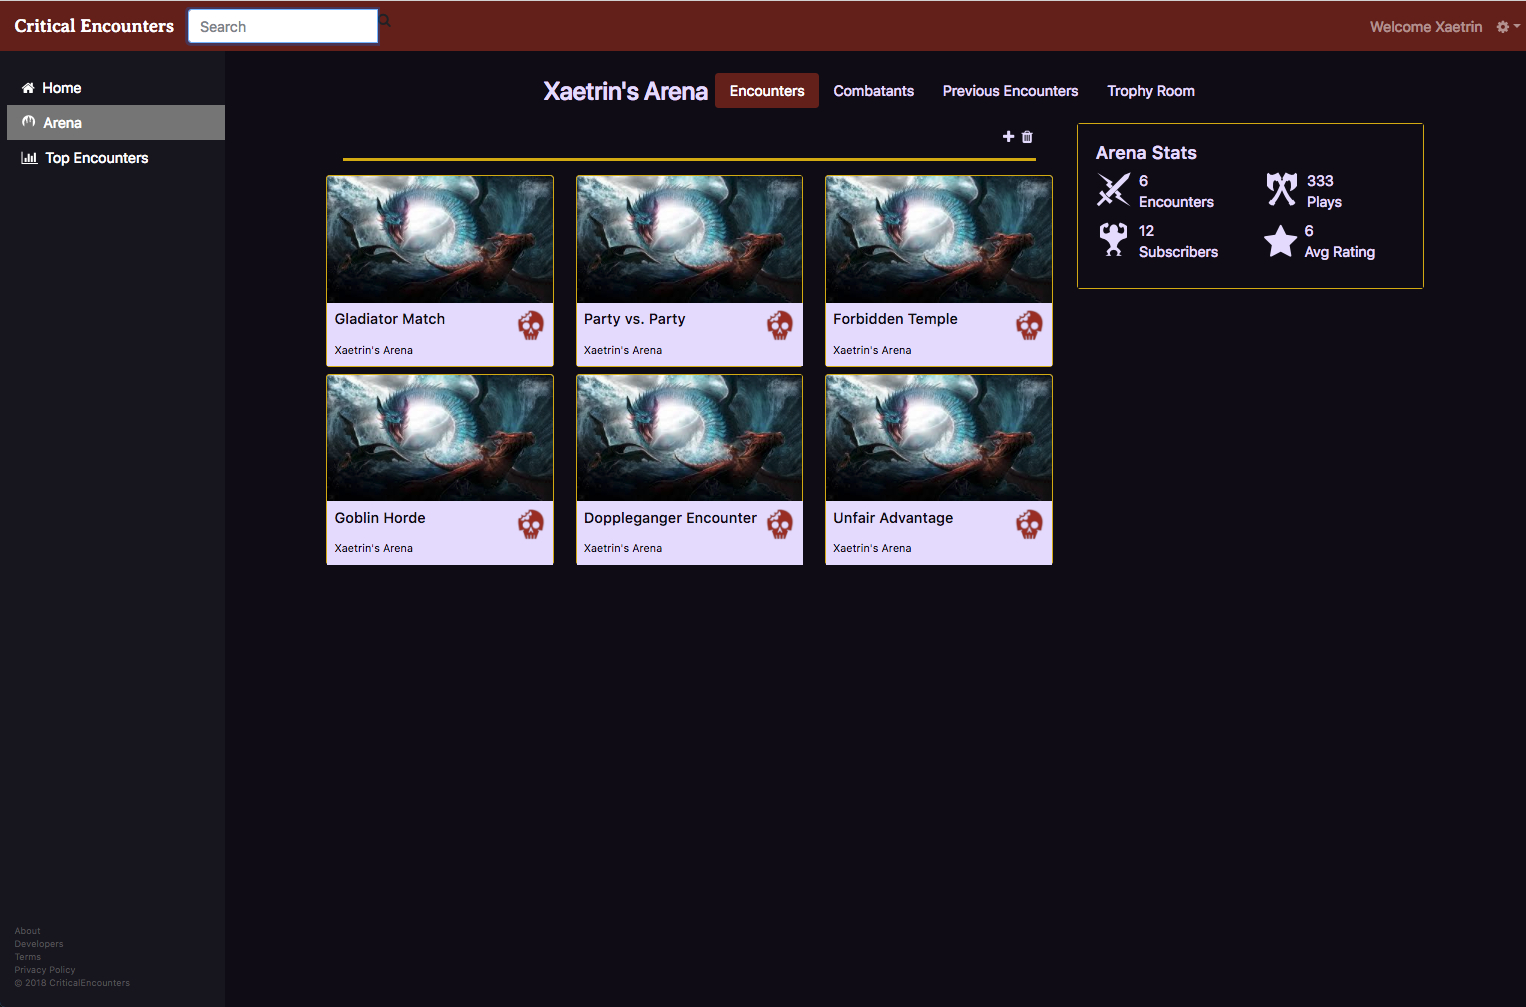
\includegraphics[scale=.20]{arena}
		\caption{Arena}
		\label{fig: Arena}
	\end{figure}
	Each Critical Encounters user is provided a page to host their published encounters for the rest of the community to access, their Arena. From the Arena page (Figure \ref{fig: Arena}) is where users are redirected to encounter creation within the Battlefield by clicking the ``Create Encounter'' button on their own Arena. Users also have the ability to edit their Arena, listing their created encounters in whatever order they wish, whether done manually or by analytics (Plays, Win Rate, Rating). At the top of the Arena page is the username and profile picture of the user tied to the Arena. The Arena presents the user's creations in a list format, with pertinent information listed alongside each encounter. Number of plays, PC win rate, overall rating, and the number of comments are shown under the encounter's title and description, and to the right of a screenshot or preset image of the encounter board itself. To the right of the encounter list, additional data on the user's arena is supplied: 
	\begin{multicols}{2}
		\begin{itemize}
			\item Number of Encounters
			\item Number of Subscribers
			\item Number of Plays
			\item Average Encounter Rating
		\end{itemize}
	\end{multicols}
	Below that, a Heat Map figure illustrates how well each class performs (Wins/Losses) in the encounters in the Arena.
	\newpage
	\section{Encounter Page}
	\begin{figure}[H]
		\centering
		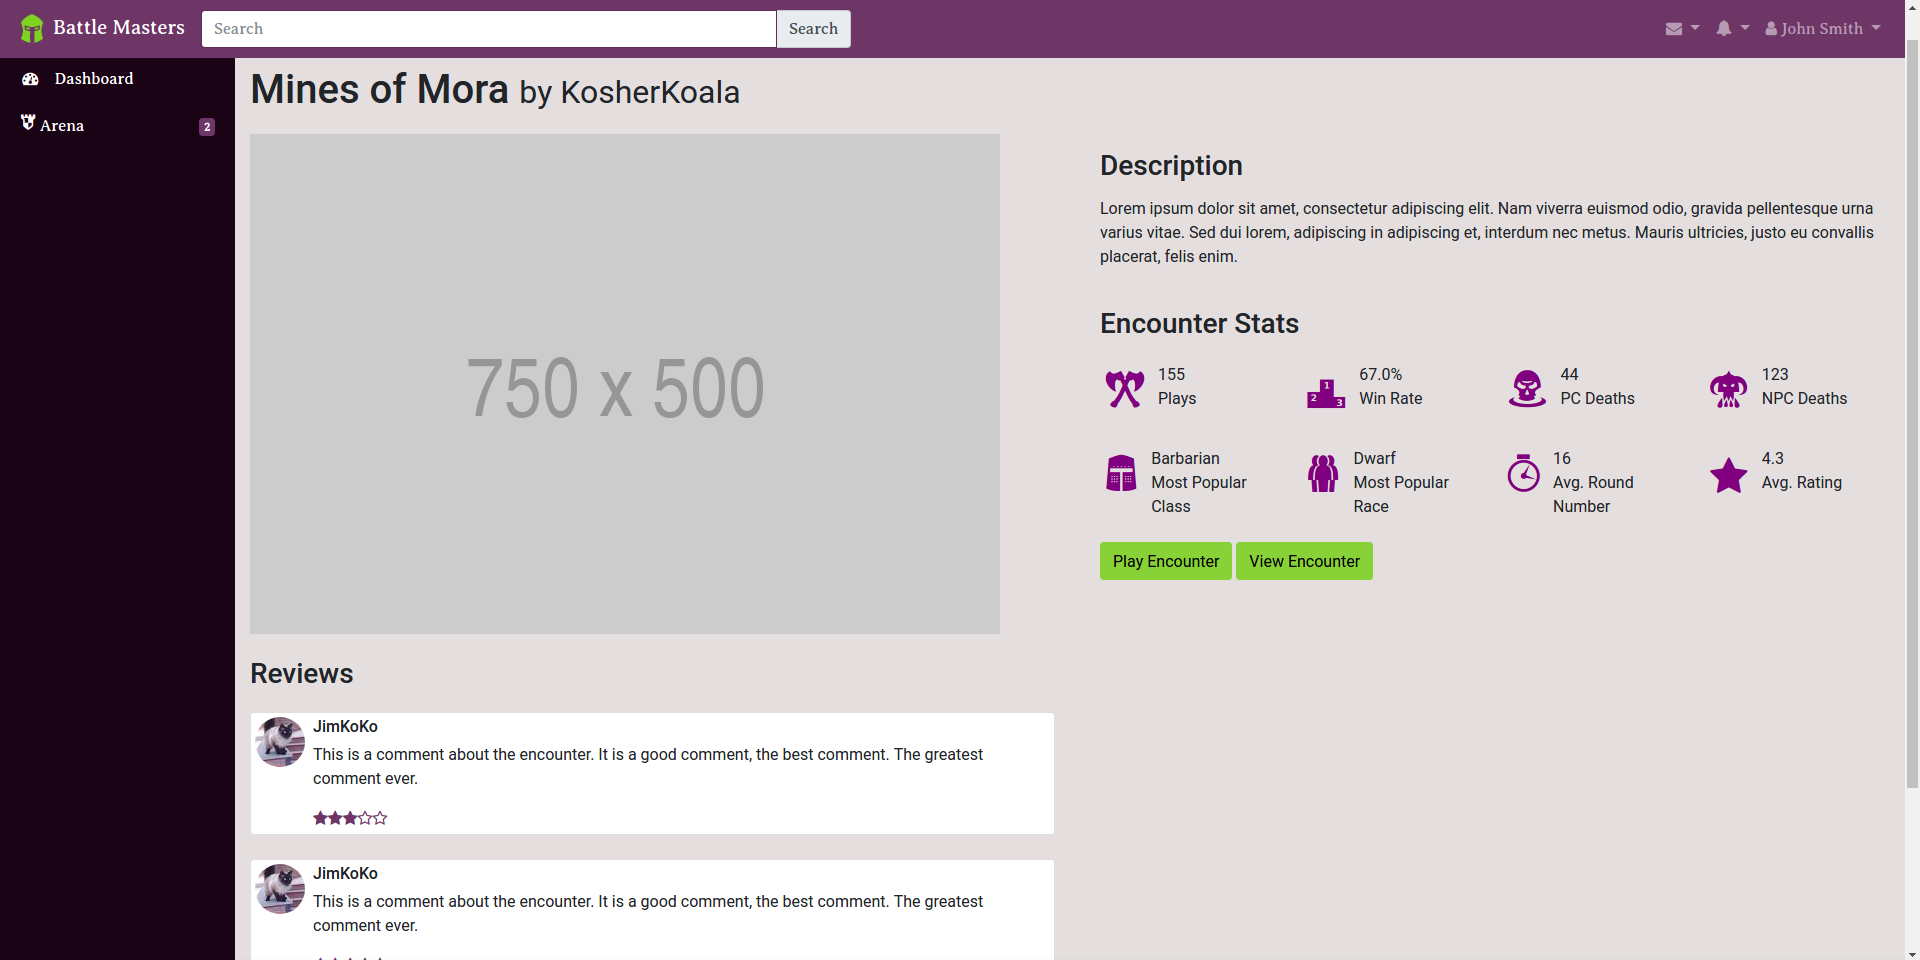
\includegraphics[scale=.20]{encounter}
		\caption{Encounter Page}
		\label{fig: Encounter Page}
	\end{figure}
	Each encounter created in Critical Encounter is given an encounter page, from which user's navigate to in order to start playing the encounter. At the top of the encounter page is the encounter's name, followed by the username of its' creator. Below is a screenshot or preset image of the encounter board, and the creator's description of the encounter hangs to the left of the image. The encounter page also presents the user with statistics related to the encounter:
	\begin{multicols}{2}
		\begin{itemize}
			\item Number of Plays
			\item Win Rate
			\item Number of PC Deaths
			\item Number of NPC Deaths
			\item Most Popular Class
			\item Most Popular Race
			\item Average Number of Rounds
			\item Average Rating
		\end{itemize}
	\end{multicols}
	\newpage
	\section{Battlefield}
	\lipsum[3]
	\newpage
	\section{Color Scheme}
	\begin{figure}[H]
		\centering
		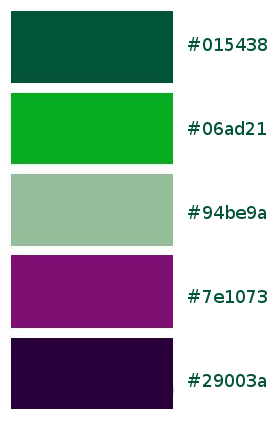
\includegraphics[scale=.5]{colors}
		\caption{Color Scheme}
		\label{fig: Color Scheme}
	\end{figure}
	\lipsum[4]
	\newpage
	\section{Icons}
	Most of the icons we utilize will be provided by the free icon APIs font-awesome and rpg-awesome. Additional icons will be acquired through Game-Icons.net.
	\begin{itemize}
		\item 
\includegraphics[scale=.06]{dashboard_icon}
		The Dashboard icon is used in the navbar and on the Dashboard itself to indicate where the user is on the site.
		\begin{figure}
			\caption{Dashboard Icon}
			\label{fig: Dashboard Icon}
		\end{figure}
		\item 
\includegraphics[scale=.03]{arena_icon}
		The Arena icon represents the users' Arena and is used in the navbar and on the Arena page itself to indicate where the user is on the site.
		\begin{figure}
			\caption{Arena Icon}
			\label{fig: Arena Icon}
		\end{figure}
		\item 
\includegraphics[scale=.03]{plays_icon}
		The plays icon is placed next to the number of plays that an Encounter or Arena has had. It appears on the users' Arena as well as on the Encounter Page itself.
		\begin{figure}
			\caption{Plays Icon}
			\label{fig: Plays Icon}
		\end{figure}
	\end{itemize}
	\subsection {Logo}
	\begin{wrapfigure}{l}{0\textwidth}
		
\includegraphics[scale=.5]{logo-large}
		\caption{Critical Encounters' Logo}
		\label{fig: Critical Encounters' Logo}
	\end{wrapfigure}
	We wanted the logo design to accompany the overall UI of the website with a simplistic design, while also representing the RPG aspect of Critical Encounters. We decided on a helmet because it gave a little more of a human feel, we thought swords or other weapons would be too inanimate. We chose the green color so the logo will "pop" with most backgrounds.This logo can also be easily scaled to fit most container sizes.
\newpage
\chapter*{Technical Goals}
\stepcounter{chapter}
\addcontentsline{toc}{chapter}{Technical Goals}
	\section{Overall Goals (Requirements???)}
	\section{Project Timelines}
	Our project takes place over two full semesters as part of the courses Senior Design I and Senior Design II. There are two major milestones that correspond to the end of each semester. The primary deliverable for semester one will be the final design document. Although the final design document will be the primary focus of semester one, we will also be focused on making small but meaningful progress in our implementation in order to have a solid head start for the second semester. The final deliverable for semester two will be the completed system as described in the design document. 
	
	There will be a period of time between the two semesters in which no milestones are listed. However, this time will be used to make small foundational progress towards the implementation of the final system in order allow for the smoothest transition into the implementation phase as possible. 
	
	Each semester will be broken down into a smaller organized list of milestones. Each of these milestones will have a deadline which should be met. The list of these milestones is show in Table \ref{table: milestones}
	
	\begin{table}[H]
		\begin{center}
			\begin{tabular}{ |c|c| } 
				\hline
				Milestone: & Completion Date: \\
				\hline
				Define Requirements/Initial Project Proposal & 10/9/2017 \\
				Verify Requirements & 10/16/2017 \\
				Decide Development Model & 10/23/2017 \\
				Define Sections & 10/30/2017 \\
				First Project Presentation Draft & 11/13/2017 \\
				Assign Design Document Sections & 11/20/2017 \\
				Senior Design Final Document & 11/29/2017 \\
				Web App Board And Gameplay & 1/9/2018 \\
				AI Prototype For DM and PC & 1/18/2018 \\ 
				PC Save/Load & 1/25/2018 \\
				Encounter Save/Load & 2/1/2018 \\
				Save/Load To Server & 2/12/2018 \\
				Browser Search And Play & 2/28/2018 \\
				Browser Ratings/Follows & 3/5/2018 \\
				Encounter Tester Implementation & 3/12/2018 \\
				Encounter Tester Statistics/Feedback & 3/19/2018 \\
				Advanced AI (Additional Settings, Counters) & 3/30/2018 \\
				Encounter Tester Advanced Features & 4/9/2018 \\	
				\hline
			\end{tabular}
		\end{center}
		\caption{Milestones} \label{table: milestones}
	\end{table}
	
	\section{Communication}
	\section{Research}
	\section{Budget}

\newpage
\chapter*{Server Design}
\stepcounter{chapter}
\addcontentsline{toc}{chapter}{Server Design}
	\section{User Roles}
	\section{Node.js}
	\section{Express.js}
	\section{Multer}
	\section{Mongoose}
	\section{Server Sequence Diagrams}

\newpage
\chapter*{Database Design}
\stepcounter{chapter}
\addcontentsline{toc}{chapter}{Database Design}
	\section{Schemas}
		\subsection{User Schema}
		\subsection{Arena Schema (HAHA THAT RHYMES)}
		\subsection{Encounter Schema}
		\subsection{Combatant Schema}
		\subsection{Obstacle Schema}

\newpage
\chapter*{Application Design}
\stepcounter{chapter}
\addcontentsline{toc}{chapter}{Application Design}
	\section{Design Patterns}
	\section{Accessibility}
	\section{Types of Views and Controllers}
	\section {Battlefield Modes}
		\subsection{Game Mode}
			This is the main mode available in DMBD. In this mode users will be able to play, simulate, and view and gather data about their and other user's encounters.
			\subsubsection{Roles}
				\paragraph{Player}
					Player is in control of a single player character and can either control his character directly in combat or apply an AI to his player character. every round the player will perform his/her character's actions on its turn. Once complete the AI will simulate all other combatant's turns and refresh the battlefield. Once the encounter is complete the player will be able to view his character's stats and results from the encounter.
				\paragraph {Game Master} Controls multiple combatants against a one or more player characters. The game master on each turn can choose to either simulate the combatant's turn or perform the actions on the combatant's turn manually using the AI. After the encounter has completed there the game master will be able to review the encounter stats and results.
				
		\subsection{Creation Mode}
			\subsubsection{Roles}
				\paragraph There is only one role available for the Creation Mode: Creator. In this mode the user will be able to design their own encounters using the Encounter Creator Tools. Users will be able to add obstacles and combatants, as well as customize the combatants stats and AI presets. Once the user has completed creating the encounter the user may either publish the encounter, and perform Encounter Validation process or keep the encounter private for personal or invite use.
	\section{Map / Environments}
	\section{Turn Structure / Order}
	Combat using the d20 System is composed of rounds in which each combatant in the encounter has one turn.  A round lasts 6 seconds in game time, during which all combatants act on their respective turns. Where a combatant's turn resides chronologically in a round is determined by the combatant's initiative roll (a combination of a dice roll and applicative bonuses). A turn it self is composed of 6 parts: Action(s), Bonus Action, Movement, Free Action, and Bonus Action, Reaction.
	\begin{itemize}
		\item Action
			\begin{itemize}
				\item The main action of a turn, every combatant has one or more per turn
				\item Ex. Attack, Cast a Spell, Dash, Disengage, Hide
			\end{itemize}
		\item Bonus Action
			\begin{itemize}
				\item An action gained by a feature, spell, or other abilities
				\item Ex: The Cunning Action feature allows a rogue to take a Bonus Action to hide, dash, or disengage
				\item Max one Bonus Action per turn
			\end{itemize}
		\item Movement
			\begin{itemize}
				\item Combatant can move the number of spaces equal to its speed (with applicaple bonuses) divided by five
				\item Some combatants also have swim and flight speeds that they can use as their movement action
				\item Multiple environmental restraints on this: Difficult terrain, attacks of opportunity
			\end{itemize}
		\item Free Action
			\begin{itemize}
				\item Interact with one object or environment 
				\item Ex: Open a door, you could draw your weapon
				\item interaction with more than one action requires the use of an action
			\end{itemize}
		\item Reaction
			\begin{itemize}
				\item Combatant has one of reaction in every round of combat
				\item Can happen anytime during the round, doesn't have to be combatant's turn
				\item Ex. Cast reaction spell, attack of opportunity
			\end{itemize}
	\end{itemize}
	\section{Computer Opponent (A.I.)}
	Since the combat simulator will support only one user, it will be necessary to implement an A.I. capable of controlling either the GM or PC actions. The A.I. must be versatile enough to play either role with an average measure of competency. It is not important that the A.I. makes the optimal tactical decision per action, as this would conflict with the role-playing nature of the D20 system. Instead, the A.I. will have various personality presets, which will be used to guide the A.I. decision making to better match the personality of the person or creature that it is controlling. In some cases, this may lead to a suboptimal action being taken intentionally. Such behavior would be left up to the creator of the encounter and the personality they select for each creature they place in it.
	
		\subsection{A.I. Responsibilities}
		If the user is controlling the PCs, the A.I. will control all other allied, neutral and hostile units on the board that are not one of the PCs. If the user is controlling the GM, the A.I. will control the PCs only. This follows the traditional design of the DnD 5e combat rules. In the case that the A.I. must control two units, one that is hostile to the PCs and one that is in alliance with them, the A.I. will take the actions that are in the best interest of the unit it is controlling for that action, regardless of whether or not that action is in the interest of the side that the A.I. is playing for. 
		
		\subsection{Challenges}
		Combat in DnD 5e allows for an extreme degree of improvisation due to the nearly infinite range of possibilities offered by the games emphasis on 'role-playing.' Role-playing is when a human player makes in-game decisions as if they are living in the mind of their character instead of their own. As an extension of this fact, players can choose to take actions that are not explicitly defined in the rule book and are instead, made up on the spot. The range of possible actions a player can make is as robust as the physics of the universe in which the game is taking place allows. 
		
		Most frequently, human players who are role-playing will disregard information that their in-game character would not know, such as information received from other human players whose corresponding characters are not within earshot and as such, are not able to talk to the player's in-game character. Another example of an event like this is if player character B is losing a battle in a remote location to player character A, the human controlling player character A would know that player character B is in trouble, but would not choose to rush to the aid of player character B since their player character has no way of knowing that player character B is in danger. Another way players role-play is by making decisions based on not what they personally want to do, but what their player character would do based on the personality and moral alignment of that player character.
		
		Players are also able to role-play when deciding specifically what their in-game actions \textit{are}. When in combat, DnD 5e provides are set of rules for what actions can take place and in what order as is typical of most tabletop board games. However, besides taking one of the basic actions defined in the game rules, players can also choose to make a 'custom' action that is specific to the in-game scenario. This usually takes the form of a player dictating to the GM what they \textit{want} to do, and the GM deciding whether that is acceptable based on their interpretation of the game rules. In this case the GM acts as a translator by attempting to compare the 'custom' action described by the player into something that fits into the general rule set of the game. 
		
		An example of such a scenario would be a player who instead of firing their bow at an enemy goblin, instead explains to the GM that they want to fire their bow at boulder hanging precariously over a cliff edge, in an attempt to create some sort of avalanche. The GM would then have to decide whether the character is physically capable of doing the described action, and what dice roles the player should make in order to succeed. The GM would then narrate the results of the player's custom action. Obviously, this specific scenario is not defined in the rule book, so the GM is in complete control of the results. If the player does not get a very successful role, the GM may decide to rule that the boulder falls as planned, but rolls off course and damages the player or their allies. Alternatively, the GM may say that the player's arrow simply misses, and no other effects occur. These highly customizable instances of role-playing have the capacity to have dramatic impact on gameplay, and is limited only to the player's creativity and improvisational skills. 
		
		It is the duty of the GM to make sure that none of these actions are too ambitious. For example, a GM would most likely decline a player's request to "instantly defeat all enemies on the field by picking up and throwing a mountain at them." Such an action would be nonsensical, and would far exceed the player characters capabilities. Inexperienced players will generally tend to use less of these improvisational actions, opting instead to stick to the basic actions defined in the rulebook, but highly experienced players will often come up with highly creative and interesting actions. It is important to remember that these custom actions are not inherently more powerful than any of the basic actions defined in the rulebook. They merely exist to add a level of 'flair' to the actions that unfold during play. It is more engaging for a player to stretch their imagination and come up with exciting or hilarious actions as they get into the role of their character. 
		
		 This level of role-play is effectively impossible to implement in any current A.I., since a human player is necessary to imagine unique contextual actions, and a human GM is necessary to judge them and decide on the results. We address this challenge by limiting all actions within the combat simulator to those that are well defined by the rule set for DnD 5e. This is not a major limitation, as the provided actions are more than enough for any encounter to be played. Additionally, since it is the goal of the GM to moderate the effectiveness of custom actions by the players, a player's tactical efficiency is not reduced by limiting them to only well-defined actions. 

		Additionally, to address the challenge of character 'personalities,' we choose to allow encounter creators to assign a personality preset to any unit on the battlefield. This personality preset will adjust the weighting of the decision making process, causing the unit to \textit{appear} to prefer certain actions. For example, a 'brute' personality will frequently choose to attack with melee even if it is not the most optimal decision, as this is the nature of role-play. Whether or not to make use of these personalities is entirely up to the user, and how they believe their encounters should feel. 
		
		\subsection{Decision Making}
		
		\subsection{Unit Personalities}
		In order to capture the spirit of the game being simulated, we allow for users to assign preset personalities to units during encounter creation in order to further customize the way those units will behave in combat. This is necessary to simulate the way in which a GM will often manipulate units in combat to act appropriately given their level of intelligence and tactical ability, as well as to increase the tension and excitement of the players taking part in the encounter. 
		
		Players creating an encounter will be able to select the personality of \textit{any} unit that they themselves have placed in the encounter. This includes all GM controlled units as well as any PC's the encounter creator places, if any. It is necessary to select a personality for any player characters in the encounter since users are able to play as the either the PCs or the GM side. In the case a user is currently controlling the GM, the A.I. will need a personality with which to base the PC's behavior. If the user is controlling the PCs and the encounter creator has defined a personality for one of the PCs the user is controlling, the personality will not take effect. It is up to the user to decide if they want to play along with the PC's given personality, or play their own way. 
		
		If a personality is selected that alters the decision making process for an A.I. controlled unit, we will apply a weighting scheme to each calculation during the decision making process in order to reflect the unit's preference for certain options. These weights will generally manifest as a multiplier to the final outcome of each of the damage, support, and crowd control calculations. If we want a personality to be, for example, barbaric, we may choose to apply a 1.5 multiplier to the potential damage calculation, and a .5 multiplier to potential support calculations. This will result in the algorithm selecting support actions far less frequently than damaging actions. 
		
		\subsection{(Future Work?) Intelligence Based Decision Making and Personalities}
		As proposed, the unit personalities system will be capable of modifying the types of actions the A.I. chooses for each unit on the battlefield. This allows of to create personalities that have preferences for which \textit{types} of abilities to choose, however, the algorithm will still pick what it believes to be the most optimal actions while abiding to that unit's preference. 
		
		Experienced GMs will take a multitude of factors into account when choosing an action for any unit under their control. One of these factors is the units level of intelligence. A creature with a high level of intelligence will intuitively have greater tactical capacity. Currently, there is no proper way to reflect this with our unit personalities system. 
		
		%Challenges ... 
		
		%Possible Solutions ...
		
		\subsection{(Future Work?) Custom 'Role-Play' Actions}
	
	\section{Encounter Diagnostics (Stress-Tester)}
	The encounter diagnostics tool, or stress-tester, will be a feature available to users of the website to evaluate their encounter designs and receive highly detailed evaluation based on a variety of metrics. Because combat in DnD5e is quite extensive and highly open ended, it is unlikely that a user seeking to create a well balanced and fluid encounter will be able to do so with some trial and error. Instead of manually playing the encounter repeatedly with multiple variations to check for weaknesses in the design, users will be able to run the built in encounter diagnostic tool to automatically generate useful information regarding their encounter. 
	
		\subsection{Restrictions}
		The encounter diagnostic tool will require as input a valid encounter that has passed verification. A valid encounter is one that has at least the minimum amount of components necessary for an encounter between the player characters and game master to be simulated. For an encounter to be verified, the creator of the encounter must succeed against a computer controlled game master at least once while controlling a party of player characters that meet the designated restrictions set by the encounter creator.  
		
		This requirement is imposed as the diagnostic tool is not meant to be used during the design process to help a creator shape their encounter. It would require additional functionality to enable the encounter diagnostic tool to work correctly on partially finished encounters and additional functionality to process the resulting data such that it is useful to the encounter creator in designing the remainder of the encounter. 
		
		Additionally, the encounter must have passed verification in order to strengthen the notion that all final encounters must have at least one solution found explicitly by a human user. This is to prevent encounter creators from using the diagnostic tool to figure out if their encounter is possible without having to test or verify it themselves. 
		\subsection{Interface}
		The user will be able to access the interface for the encounter diagnostic tool from within the encounter creator. The encounter diagnostics option will only be available on encounters that the user has created. Once the user has selected an encounter to perform encounter diagnostics, they will be prompted to enter details necessary to configure the tests. 
		
		\subsection{Diagnostic Measurement}
		When activated, the encounter diagnostic tool will generate a set of valid party member compositions that meet both the restrictions of the encounter as well as the additional restrictions provided by the user during configuration. A party composition is a collection of player characters that will be placed on the field of play at the start of the encounter. The diagnostic tool will generate one party composition per iteration of the test. Once all party compositions are generated, the diagnostic tool will simulate the encounter one time for each party composition. 
		
		The simulation will consist of each member of the party being placed in the user designated spawn positions for the encounter. Once all player characters are placed, both PC and GM turns will be taken by the A.I. until either side meets their win condition, at which point the board is reset and the next party composition is tested. Once all party compositions have been tested, the diagnostic tool serves the results of the tests to the user.
		
		 During each test , statistics relating to the performance of each entity in the encounter will be tracked in order to provide metrics by which the user can evaluate their encounter. Statistics that will be tracked include the following:
		 
		\begin{itemize}
			\item Number of kills/deaths for each non-PC entity in the encounter
			\item Number of kills/deaths by each "class" of PC
			\item Overall win rate of PC vs GM
			\item Damage per ability used
			\item Location of each kill made on the map
			\item Turn count
		\end{itemize}
		
		\subsection{Results and Presentation}
		One all simulations are complete and the data has been collected, it must be processed into a form that is quick and easy to understand. Each statistics that was tracked on a per-encounter basis will be aggregated into an average value and presented to the user in a separate window. These average values will highlight at a glance measurements such as the average length of each encounter, which enemies are the most dangerous, how difficult the overall encounter is, and which abilities are the most effective in the encounter. Additionally, a heat map will be generated using the location of kills made on the map across all simulations. This heat map will indicated to the user the general flow of combat, which can be used to help fine tune the encounter and improve overall quality. 
		
	\section{Encounter Browser}
	\section{Encounter Creator Tools}
	\section{Storyboards}
	\section{Version Control}
	\section{Data Processing from API (WHAT DOES THIS MEAN???)}

\newpage
\chapter*{Research}
\stepcounter{chapter}
\addcontentsline{toc}{chapter}{Research}
	\section{MEAN Stack}
	\begin{figure}[H]
		\centering
		
\includegraphics[scale=.2]{meanStack}
		\caption{Mean Stack Logo}
		\label{fig: Mean Stack Logo}
	\end{figure}
	The creation of developer tools like MongoDB, Express.js, Angular.js, and Node.js (otherwise known as the MEAN stack) forge a collection of technologies that allow for JavaScript utilization when developing a web application. The culmination of these technologies build off each other while staying modular. This can allow for a head start in the initial stages of development with scaffolding for all of the main tools in the MEAN Stack.
	
		\subsection{Altered MEAN Stack}
		After scouring the internet for alternatives, we found that Meteor.js is a welcome alteration to the MEAN Stack implementation. Meteor.js is another API that allows for focus on JavaScript coding in development across front-end and back-end applications. While it is a bit more heavyweight than the Express.js framework, on the Node.js platform, Meteor.js is designed to accelerate development of web applications. As an extention of the MEAN Stack, this is achieved just the same, by having a number of components pre-configured out-of-the-box, which allows for an enormous head-start in development.
			\newpage
			\subsubsection{MongoDB}
			\begin{wrapfigure}{r}{0\textwidth}
				
\includegraphics[scale=0.05]{mongoDB}
				\caption{MongoDB}
				\label{fig: MongoDB}
			\end{wrapfigure}
			We decided to utilize MongoDB, a NoSQL database that is an essential part of the MEAN Stack. There are quite a few reasons to opt for a more modern approach to constructing databases, for instance, the structure and data type in schemas in a SQL database are fixed. To store information about a new data item, the entire database must be altered, during which time the database must be taken offline. With this project taking on an agile approach in its’ development cycle, and a database being so essential to early development with the implementation of the many items, rules, and class/monster types that are available, starting that database and being fixed in the schemas we create could cause a slow in development later in the cycle when changes are made. However, when using a NoSQL database like MongoDB, insertion of data is allowed without any predefined schema. This means development and integration of code is faster and more reliable. A document database model for data storage that we can adopt when using a NoSQL database is another benefit to using MongoDB, because it best fits the way that information is organized while using the d20 Game System.
			\newpage
			\subsubsection{Meteor.js}
			\begin{wrapfigure}{l}{0\textwidth}
				
\includegraphics[scale=.2]{meteorJS}
				\caption{Meteor.js}
				\label{fig: Meteor.js}
			\end{wrapfigure}
			Meteor.js is a full-stack JavaScript platform for developing modern web and mobile applications. Like much of the API's we are implementing in the development of this web application, Meteor allows for coding in JavaScript across the front-end and back-end side of development. The biggest advocate for including Meteor in our project is its' focus on development speed. All server-side applications are handled in the development of the client-side. That is to say, when developing client-side applications, any server-side necessities are taken care of by Meteor.js’ ability to redirect data in the background. The scaffolding that is included directly out of install with Meteor, such as a fully configured MongoDB database and integration with Angular while still having a fully integrated stack, is a leap forward in the development cycle of this project, so we will have more time for fine-tuning features and performance of the web application later. Meteor also uses web sockets instead of HTTP-style pull requests, so the server pushes updates to the client when new data is available, and the client renders that data. This allows Meteor to implement "hot-pushing", where developers can push updates the client even while it a user is in the middle of a session. Any fixes or improvements can be pushed without the user even knowing.
	
			\subsubsection{Node.js}
			\begin{wrapfigure}{r}{0\textwidth}
				
\includegraphics[scale=0.06]{nodeJS}
				\caption{Node.js}
				\label{fig: Node.js}
			\end{wrapfigure}
			Node.js is a runtime application that starts small but grows more and more useful as additional modules are implemented. There are a few reasons why it is the first choice when building a web application like this project. Node allows for JavaScript coding on the server side of a website or web application. This results in the idea that code can be written once, but ran on both the server and the client browser, optimizing which functions would give users faster response times while also lifting a bit of work for the server. Writing server-side code in JavaScript using Node also keeps the logic and code very similar across the server and client. Also, Node uses an asynchronous even driven mode, so that when a task is performed, other tasks are not prevented from being run.
	
			\subsubsection{Angular 4}
			\begin{wrapfigure}{l}{0\textwidth}
				
\includegraphics[scale=.25]{angular_js}
				\caption{Angular 4}
				\label{fig: Angular 4}
			\end{wrapfigure}
			\lipsum[1]
			Angular 4 is a font-end TypeScript framework used for developing frontend web and mobile based applications. We will be using Angular 4 for the fontend of our web app.  
	
			\subsubsection{Bootstrap 4}
			\begin{wrapfigure}{r}{0\textwidth}
				
\includegraphics[scale=0.1]{bootstrap4}
				\caption{Bootstrap4}
				\label{Bootstrap 4}
			\end{wrapfigure}
			Bootstrap is a HTML, CSS, and JS framework used for building responsive, mobile compatible web sites and applications. Bootstrap was an obvious choice for out front end development. It has extensive documentation and resources available. Also with its new v4 update Bootstrap is more useful then ever. Our front end team already has extensive experience with Bootstrap so it should be easy to get the front end up and running. One issue we had to address is Bootstraps dependency on jQuery. jQuery is JS API whose functions can sometimes interfere with Angular 4's TS functions. To avoid these issues we decided to avoid using jQuery entirely and use ng-bootstrap instead witch performs all of bootstraps jQuery functions entirely in Angular 4.
			
			
	\section{RESTful}
	\section{Game A.I.}
		\subsection{Pathfinding}
		\subsection{Basic Rule Following (Non-A.I. Computer Opponent)}
		\subsection{Decision Trees}

\newpage
\chapter*{Appendix}
\stepcounter{chapter}
\addcontentsline{toc}{chapter}{Appendix}

\newpage
\stepcounter{chapter}
\addcontentsline{toc}{chapter}{Figures}
\listoffigures

\newpage
\stepcounter{chapter}
\addcontentsline{toc}{chapter}{Tables}
\listoftables

\newpage
\chapter*{References}
\stepcounter{chapter}
\addcontentsline{toc}{chapter}{References}
	
\end{document}